\subsubsection{Test \ref{test4}, Both BFS and DFS searches return correct values for an empty graph.}
Input:  On an empty graph, click on the \enquote{Depth First Search} button, observe the message in the status bar, then click on the \enquote{Breadth First Search} button, and observe the message in the status bar.
\newline
\newline
Expected output: For the Depth First Search button, the status bar should display \enquote{DFS:}, with no additional content. For the Breadth First Search button, the status bar should display \enquote{BFS:} with no additional content.
\begin{figure}[ht]
    \centering
    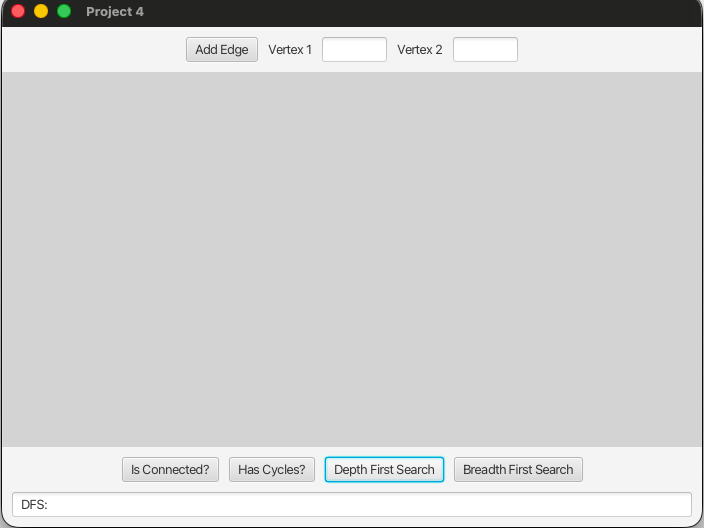
\includegraphics[width=0.65\textwidth]{images/test4-dfs.png}
    \caption{test \ref{test4} - Depth First Search button}
\end{figure}
\begin{figure}[ht]
    \centering
    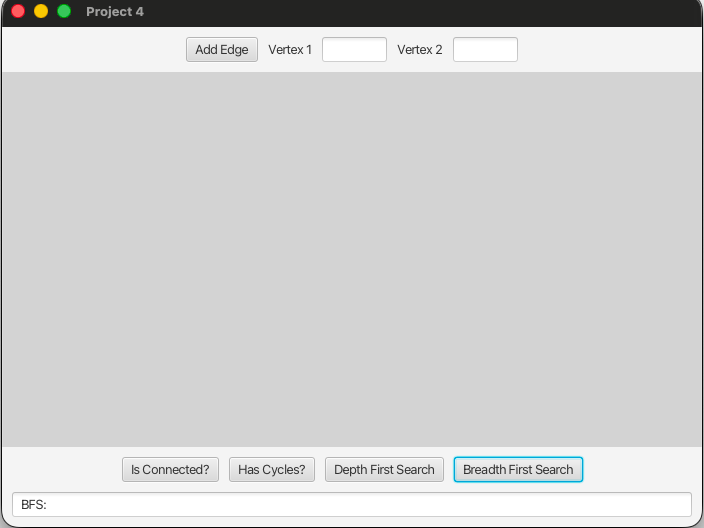
\includegraphics[width=0.65\textwidth]{images/test4-bfs.png}
    \caption{test \ref{test4} - Breadth First Search button}
\end{figure}
